
\vspace{-2mm}

\section{Overview of Heavy-Tailed Self-Regularization}
\label{sxn:theory-review}

\vspace{-1mm}

%In this section, we will briefly review results from Universality that will be relevant for our analylsis.
We review Martin and Mahoney's Theory of Heavy-Tailed Self-Regularization (HT-SR)~\cite{MM18_TR,MM19_HTSR_ICML}.
%%\michael{We need to push the other 10 pager to the archive, without the supplementary information}

Write the Energy Landscape (or optimization function) for a typical DNN with $L$ layers, with activation functions $h_{l}(\cdot)$, and with $N\times M$ weight matrices $\mathbf{W}_{l}$ and biases $\mathbf{b}_{l}$, as:
\begin{equation*}
%PRESQUISH% E_{DNN}=h_{L}(\mathbf{W}_{L}\times h_{L-1}(\mathbf{W}_{L-1}\times h_{L-2}(\cdots)+\mathbf{b}_{L-1})+\mathbf{b}_{L})  .
E_{DNN} \hspace{-1mm} = \hspace{-1mm} h_{L}(\mathbf{W}_{L}\cdot h_{L-1}(\mathbf{W}_{L-1}\cdot h_{L-2}(\cdots)+\mathbf{b}_{L-1})+\mathbf{b}_{L})  .
%\label{eqn:dnn_energy}
\end{equation*}
%WLOG,
Typically, this model would be trained on some labeled data $\{d_{i},y_{i}\}\in\mathcal{D}$, using Backprop, by minimizing the loss $\mathcal{L}$.
For simplicity, we do not indicate the structural details of the layers (e.g., Dense or not, Convolutions or not, Residual/Skip Connections, etc.). 
Each layer is defined by one or more layer 2D weight matrices $\mathbf{W}_{l}$, and/or the 2D feature maps $\mathbf{W}_{l,i}$ extracted from 2D Convolutional (Conv2D) layers.
(We have not yet analyzed LSTM or other complicated Layers.) 
A typical modern DNN may have anywhere between 5 and 5000 2D layer matrices.%
\footnote{%
%Some notational conventions:
For each Linear Layer, we get a  single $(N\times M)$ (real-valued) 2D weight matrix, denoted $\mathbf{W}_{l}$, for layer $l$.  
This includes Dense or Fully-Connected (FC) layers, as well as 1D Convolutional (Conv1D) layers, Attention matrices, etc.
We ignore the bias terms $\mathbf{b}_{l}$ in this analysis. 
%XXX.  WHY, WHAT.   
Let the aspect ratio be $Q=\frac{N}{M}$, with $Q\ge 1$.
For the Conv2D layers, we have a 4-index Tensor, of the form $(N\times M \times c\times d)$, consisting
of $c\times d$ 2D feature maps of shape $(N\times M)$.    
We  extract $n_{l}=c\times d$ 2D weight matrices $\mathbf{W}_{l,i}$, one for each feature map $i=[1,\dots,n_{l}]$ for layer $l$.
%One could construct matrices in other ways.
}
   

\paragraph{Heavy-Tailed Empirical Spectral Distributions.}
%
%By Universal behavior, we mean that the eigenvalue spectrum associated weight matrices 
%We can identify different Universality classes 
%
In the HT-SR Theory, we analyze the eigenvalue spectrum (the ESD) of the associated correlation matrices~\cite{MM18_TR,MM19_HTSR_ICML}.
From this, we can characterize the amount and form of correlation, and therefore implicit self-regularizartion, present in the DNN's weight matrices.
For each layer weight matrix, of size $N \times M$, construct the associated $M\times M$ (uncentered) correlation matrix $\mathbf{X}$. 
Dropping the $L$ and $l,i$ indices, we have
$$
\mathbf{X} = \frac{1}{N}\mathbf{W}^{T}\mathbf{W}.
$$
%In theoretical treatments, $\gamma$ depends on the form of $\Probab{W_{i,j}}$, e.g., the value of $\mu$, in order to prove the existence of the limiting forms of the ESD.
%For MP theory and the Gaussian Universality class, we can set $\gamma=1$, but for the HT Universality classes, we need to set $\gamma=2/\mu$.
%Of course, empirically, we do not know the PL exponent $\mu$, or the particular Universality class, \emph{a priori}, and the data are of only finite size.
%This will be very important below. 
%For our empirical analysis, we set $\gamma=1$ and deal with these issues in an \emph{a posteriori} manner. 
%
If we compute the eigenvalue spectrum of $\mathbf{X}$, i.e., $\lambda_i$ such that
$  % $$
\mathbf{X}\mathbf{v}_{i}=\lambda_{i}\mathbf{v}_{i} , 
$  % $$
then the ESD of eigenvalues, $\rho(\lambda)$, is just a histogram of the eigenvalues, formally written as
\begin{equation}
\rho(\lambda)=\sum\limits_{i=1}^{M}\delta(\lambda-\lambda_{i})  .
\label{eqn:eigenval_hist}
\end{equation}
%
%From HT-RMT theory~\cite{XXX-XXX,XXX-XXX,XXX-XXX,XXX-XXX}, the ESD $\rho(\lambda)$ of a HT matrix will have a HT, taking the form
%% POSSIBLY REDUNDANT %% Empirically, for weight matrices of a modern well-trained production-quality DNN, the ESD nearly always exhibits Heavy-Tailed properties~\cite{MM18_TR,MM19_HTSR_ICML}.
%%SPACE%% \footnote{Older and smaller models exhibit ESD properties closer to a Spiked Covariance model, and it is possible to train DNNs to have ESDs with other properties, corresponsing to other types of implicit self regularization~\cite{MM18_TR,MM19_HTSR_ICML}.} 
Using HT-SR Theory, we can characterize the \emph{correlations} in a weight matrix by examining its ESD, $\rho(\lambda)$.
It can be well-fit to a power law (PL) distribution, given as
\begin{equation}
\rho(\lambda)\sim\lambda^{-\alpha}  ,
\label{eqn:eigenval_pl}
\end{equation}
which is (at least) valid within a bounded range of eigenvalues $\lambda\in[\lambda^{min},\lambda^{max}]$.  
%\michael{Ques: here, $\alpha$ is theoretical, while below $\alpha$ is fit, so clarify.}
%
We can determine $\alpha$ by fitting the   ESD to a PL, using the commonly accepted Maximum Likelihood (MLE) method of Clauset et al.~\cite{CSN09_powerlaw,ABP14}.
%(((
%\charles{Discuss fact the PL tails are Frechet at finite-size so only need to fit the bulk}
%\michael{Ques: clarify.}
%)))
This method works very well for exponents between $\alpha\in(2,4)$, and it is adequate, although imprecise, for smaller and larger $\alpha$~\cite{newman2005_zipf}. 
%\michael{Ques: careful, $\alpha$ (thoeretical or fitted) or $\mu$ here.}
%%MM%% The fitting method is robust in that it is reasonably insensitive to the the choice of normalization $\gamma=1$.

%% %Recent work by Martin and Mahoney
%% in our previous study of Heavy-Tailed Self Regularization (HT-SR)~\cite{MM18_TR,MM19_HTSR_ICML}, we examine the eigenvalue density
%% $\rho(\lambda)$, or Empirical Spectral  Density (ESD), of the linear weight matrices of very large number of modern, pre-trained, DNNs,
%% such as the AlexNet, the VGG series (VGG11, VGG13, ...) ,  etc. 

%% \charlesX{comments will go back in}
%% \charlesX{
%% We apply our new Theory of Heavy-Tailed Self Regularization (HT-SR) to analyze these large, pre-trained DNNs.  
%% We model \emph{the correlations} arising in the DNN layers by forming the normalized correlation matrices $\mathbf{X}=(1/N)\mathbf{W}_{L}^{T}\mathbf{W}_{L}$ 
%% for each of the individual  the layer weight matrices $\mathbf{W}_{L}$ and then studying the eigenvalue density of each $\mathbf{X}$,  $\rho(\lambda)$.
%% The HT-SR Theory lets us characterize the densities because they almost always display heavy tailed signatures,
%%  and can be fit to a Power Law, $\rho(\lambda)\sim\lambda^{-\alpha}$, with exponent $\alpha$.   And , on average,
%%  the smaller the $\alpha$, the more Self Regularization is in the DNN.  Of course, the
%%   pre-trained weight matrices  $\mathbf{W}_{L}$  themselves are not at all random because they have been trained 
%%   on very large, high quality data sets,
%%   and they behave quite differently from a random heavy tailed (i.e. Pareto) matrix.  And it is these differences we can exploit
%%   to predict trends in the generalization accuracy.}

The original work on HT-SR Theory~\cite{MM18_TR,MM19_HTSR_ICML} considered NNs including AlexNet and InceptionV3 (as well as DenseNet, ResNet, and VGG), and it showed that for nearly every $\mathbf{W}$, the (bulk and tail) of the ESDs can be fit to a PL and the PL exponents $\alpha$ nearly all lie within the range $\alpha\in(1.5,5)$.
Moreover, smaller exponents $\alpha$ are correlated with more implicit self-regularization and, correspondingly, better generalization~\cite{MM18_TR,MM19_HTSR_ICML}.
Subsequent work~\cite{MM18_unpub_work} has shown that these results are ubiquitous.
%\michael{Put ref to notebook in~\cite{MM18_unpub_work}.}
For example, 
upon examining nearly 10,000 layer weight matrices $\mathbf{W}_{l,i}$ across over 50 different modern pre-trained DNN architectures, the ESD of nearly every $\mathbf{W}$ layer matrix can be fit to a PL:
$70-80\%$ of the time, the fitted PL exponent $\alpha$ lies in the range $\alpha\in(2,4)$; and  %% (in the Moderately Heavy-Tailed Universality class, described below); and
$10-20\%$ of the time, the fitted PL exponent $\alpha$ lies in the range $\alpha< 2$.  %% (in the Very Heavy-Tailed Universality class, described below).
For example, see Figure~\ref{fig:power-law-histogram} for a histogram of results for ca. 7500 weight matrices from ImageNet.
%\charlesX{explain this plot, ref to notebook and check in.  This plot is for ImageNet, includes conv@D feature maps, lots of small alpha, but not as good a fit.}
Of course, there are exceptions: in any real DNN, the fitted $\alpha$ may range anywhere from $\sim 1.5$ to $10$ or higher~\cite{MM18_unpub_work} (and, of course, larger values of $\alpha$ may indicate that the PL is not a good model for the data).  
Still, overall, in nearly all large, pre-trained DNNs, the correlations in the  weight matrices exhibit a remarkable Universality, being both Heavy Tailed, and having small---but not too small---PL exponents. 

\begin{figure}[!htb]
   \centering
   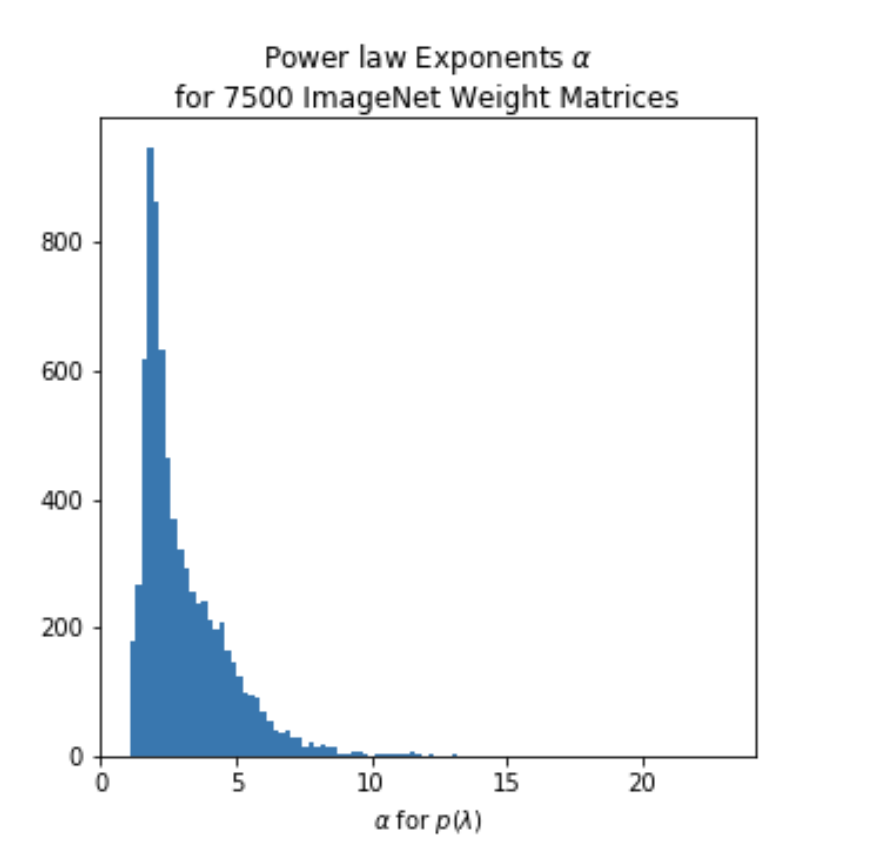
\includegraphics[scale=0.40]{img/power-law-histogram.png} 
   \caption{%
            Histogram of PL exponents, $\alpha$, fit on ca. 7500 Linear and Conv2D Layers from ImageNet. 
            The vast majority have $\alpha\in(1.5,5)$. 
            Some Conv2D layers have smaller values of $\alpha$; and larger values of $\alpha$ (up to ca. 20) exist but correspond to less reliable fits.
            }
   \label{fig:power-law-histogram}
\end{figure}





%\nred{removed this: \paragraph{Simple Random Matrix Models.} }
%One might imagine that the matrix elements of $\mathbf{W}$ are drawn from some probability distribution, e.g., a Normal $N(0,\sigma)$ distribution
%\begin{equation}
%\Probab{ W_{i,j} } \sim N(0,\sigma)
%\end{equation}
%with mean $0$ and variance $\sigma$.%
%\footnote{At the start of training, DNN weight matrices typically are approximately Normal.  This has been used by some as an analytically-tractable model for trained DNNs, but it is an empirical question whether this is a good model for very non-random matrices that arise at the end of training modern DNNs.  Empirically, it is not~\cite{MM18_TR,MM19_HTSR_ICML}.}
%%MM%% \charlesX{Our imagination here lets us derive seemingly \emph{Universal} expressions for how the correlations should behave, even though $\mathbf{W}$  itself is not at all random. }
%These Gaussian models arise in the well known Marchenko-Pastur (MP) RMT~\cite{XXX-XXX}, as well as the Spiked-Covariance model~\cite{johnstone2009}, which is a perturbative variant of MP-RMT. 
%Empirically, it is know that these Gaussian-based models are useful for understanding older, smallish Neural Networks, such as LeNet5~\cite{MM18_TR,MM19_HTSR_ICML}.
%More modern DNNs, however, display very different, more exotic,  Universal, behavior.  


\paragraph{Heavy-Tailed Mechanistic Universality.} 

%\charlesX{THIS SECTION NEEDS A LOT OF WORK}

Here, we consider the question:
what does it \emph{mean} to say that DNN weight matrices exhibit Universality? 
This answer to this---and its implications---depends on your perspective, in particular, as a Mathematician or a Physicist.

In Statistics and Applied Mathematics, Universality typically refers to properties of systems that can be modeled by random matrices.
The justification is that certain system properties can be deduced, without requiring knowledge of system details, from a few global quantities that are then used as parameters to define a random matrix ensemble~\cite{ER05,EW13}.
Of course, the DNN weight matrices are not random matrices---they are strongly-correlated objects---so it may seem odd that we can apply RMT to characterize them.

In Statistical Physics, Universality refers to a different, but related, phenomena.
It arises in systems with very strong correlations, at or near a critical point or phase transition. 
It is characterized by measuring experimentally certain ``observables'' that display HT behavior, with common---or Universal---PL exponents. 
More importantly, it indicates that a specific Universal mechanism drives the underlying physical process, e.g., Self Organized Criticality, directed percolation, etc.~\cite{SornetteBook,BouchaudPotters03}. 
For this reason, we refer to the Universality observed in HT-SR, i.e., in the ESDs of (pre-trtained) DNN weight matrices, as \emph{Heavy-Tailed Mechanistic Universality~(HT-MU)}.

For an illustration of what we mean by HT-MU, see Figure~\ref{fig:universality_diagram}. 
When we observe HT behavior in $\mathbf{W}$, or rather its correlation matrix $\mathbf{X}$, we use HT-RMT as a generative model. 
We say that we \emph{model} $\mathbf{W}$ \emph{as if} it is a random matrix, $\mathbf{W}^{rand}(\mu)$, drawn from a Universality class of HT-RMT (i.e., VHT, MHT, or WHT, as defined below). 
Of course, we do not mean that $\mathbf{W}$ is itself random in any way.
We simply use RMT as a stand-in generative model because the correlations in $\mathbf{W}^{rand}(\mu)$ resembles the correlations in  $\mathbf{W}$. 
Indeed, RMT itself does not describe the behavior of a random matrix $\mathbf{W}$ per-se, but it characterizes its correlations (i.e., the eigenvalues of $\mathbf{X}$). 
Specifically, RMT describes the ESD, $\rho_{emp}(\lambda)$, its limiting, deterministic form $\rho_{\infty}(\lambda)$, as well as the finite-size scaling and fluctuations of the maximum eigenvalue, $\lambda^{max}$~\cite{MM18_TR,MM19_HTSR_ICML}. 
So, even though $\mathbf{W}$ is not random, we expect its ESD and maximum eigenvalue to behave \emph{as if} they were drawn from some HT-random matrix $\mathbf{W}^{rand}(\mu)$.
   
%% \nred{NEED LEAD IN}
 
%See Figure~\ref{fig:universality_diagram} for an illustration.
%Due to the training process, trained DNN weight matrices are strongly-correlated; and fitting their ESDs to Eqn.~(\ref{eqn:eigenval_pl}) amounts to \emph{modeling} the correlational properties in terms of 
%known Universality classes \nred{HT-RMT}~\cite{SornetteBook,BouchaudPotters03}.

%We use HT-RMT and Universality in the way used in Statistical Physics, i.e., to derive Universal relations between empirically-measurable~quantities.

%Of course, one must do more than just observe common power law exponents to claim 
%In these cases, one can} construct scaling relations (that are then empirically evaluated) between empirically-measurable quantities

%In this case, random matrices arise since they are particularly easy-to-analyze members of a Universality class, for which these relations should hold.
%In particular, strongly-correlated DNN weight matrices are clearly not random matrices, but the latter can be used to \emph{model} the former (since, if they are members of the same Universality class, then scaling relations should hold for both).

%% \charles{%
%% EXPLAIN UNIVERSALITY, AS WE USE IT, IN THIS SECTION. 
%% NOTE: we model the ESD of X, the correlations in W, and therefore how the data has been learned. 
%% Universality of Power Law exponents is special, in the context of statistical physics / Rg theory / SOC, and different from Universality in RMT. 
%% We use RMT as a guide.
%% This section contains LOTS OF NEW information, including the 2 images and the discussion around them. 
%% Notice: the conv2D maps are VHT, not MHT.
%% So we will need an approach that crosses the 2 Universality classes. 
%% Notice: W is not itself random, but its ESD lookd like the ESD of an HT RMT.}

\begin{figure}[t]  %[!htb]
   \centering
   %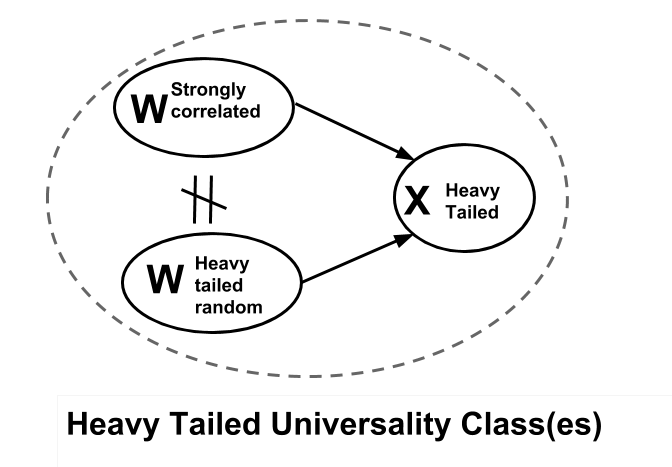
\includegraphics[scale=0.40]{img/universality_classes.png} 
   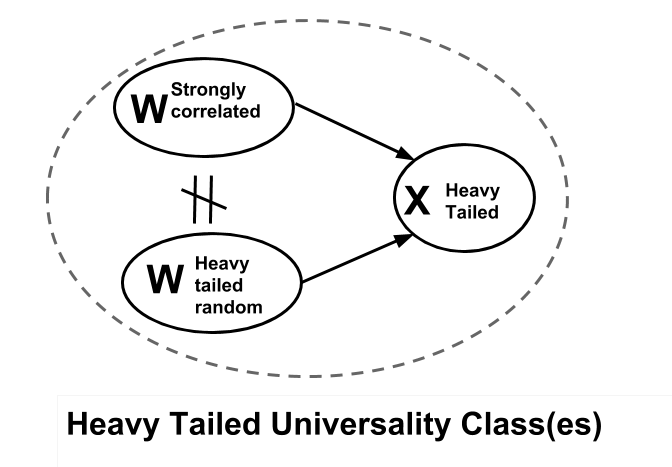
\includegraphics[scale=0.36]{img/universality_classes.png} 
   \caption{Illustration of our use of HT Universality.  
            %\michael{Charles, maybe tweak this figure to rotate and horizontally show transfer of Universal things between different matrices.}  
            A random matrix $\mathbf{W}(\mu)$ with elements drawn i.i.d. from the HT distribution of Eqn.~(\ref{eqn:ht_dstbn}) and weight matrix $\mathbf{W}^{str. corr.}$ from a modern well-trained DNN that exhibits strong correlations each arise from different generative mechanisms, and they are different.  Both exhibit similar Universality properties, as evidenced by the HT properties of the ESDs of their corresponding correlation matrices $\mathbf{X}$, and so we expect Universal properties to be similar between~them.}
   \label{fig:universality_diagram}
\end{figure}


\paragraph{Heavy-Tailed Random Matrix Theory.} 
To characterize this HT-MU behavior, we use a HT variant of RMT and use HT random matrices to elucidate different Universality classes.
Let $\mathbf{W}(\mu)$ be an $N \times M$ random matrix with entries chosen i.i.d. from
\begin{equation}
\Probab{ W_{i,j} } \sim \frac{W_{0}^{\mu}}{|W_{i,j}|^{1+\mu}}  ,
\label{eqn:ht_dstbn}
\end{equation}
where $W_{0}$ is the typical order of magnitude of $W_{i,j}$, and where $\mu>0$. 
These HT matrix models were first introduced in the Statistical Physics literature, where they are called L\'evy Matrices when $0<\mu<2$~\cite{PB94}; see also~\cite{BM97,BJNx01_TR,BJNx06_TR,heavytails2007}.
More recently, there has been mathematical work on HT random matrices~\cite{AG08,AAP09,BJ09_TR,DPS14,AT16}.
There are at least 3 different Universality classes%
\footnote{Results for $\mu=2,4$ are slightly different~\cite{SornetteBook,BouchaudPotters03}.  We don't describe them since we don't expect to be able to resolve them numerically.  Also, sometimes L\'evy matrices are split into VHT for $1<\mu<2$ and EHT (Extremely Heavy-Tailed) for $0<\mu<1$, as the properties for these two parameter regimes are somewhat different~\cite{SornetteBook,BouchaudPotters03}.}
of HT random matrices, defined by the range $\mu$ takes on:
\begin{itemize}
\item $0<\mu<2$: VHT: Universality class of Very Heavy-Tailed (or L\'evy) matrices;
\item $2<\mu<4$: MHT: Universality class of Moderately Heavy-Tailed (or Fat-Tailed) matrices;
\item $4<\mu$: WHT: Universality class of Weakly Heavy-Tailed matrices.
\end{itemize}
%%
%%\charles{ THIS SECTION REVIEWS Heavy Tail RMT, and is ALL REVIEW.  WE MUST  explain how to interpret a correlated ESD in terms of HT-RMT.  BUT be clear that this is not the whole story }
%%
%%\michael{We need to highlight how the HT Universality we use is one that crosses Universality classes, i.e., VHT and finite-sized MHT, and certainly is NOT limited to random matrices, but we use RMT to characterize certain things.}
%%


\paragraph{Heavy-Tailed, Finite-Size Relations.}

HT-RMT provides more than HT Universality classes.
It also provides simple relations between the empirical observables, e.g., the PL exponent $\alpha$ and the maximum eigenvalue $\lambda^{max}$ of each $\mathbf{W}$, with the parameter(s) $\mu$ of our generative theory, i.e, of~HT-RMT.   

%% For the VHT Universality class, the PL tail of Eqn.~(\ref{eqn:eigenval_pl}) persists in the infinite limit $N\rightarrow\infty$, for $Q$ fixed; and
%% we have the linear relation between our observed exponent $\alpha$ and the theoretical~$\mu$:
%% \begin{equation}
%% \alpha=\frac{1}{2}\mu+1  .
%% \label{eqn:alpha_mu_vht}
%% \end{equation}
%% \michael{Ques: careful, two things change here: observed versus theoretical, and matrix elements versus eigenvalues.}
%% This expression which works very well at finite size, even for very small matrices $(M,N\approx100)$.
%% %
%% For the MHT Universality class, the PL tail of Eqn.~(\ref{eqn:eigenval_pl}) vanishes in the infinite limit $N\rightarrow\infty$, for $Q$ fixed.
%% \michael{Ques: what does ``vanishes'' mean, it changes slope, and it is MP in the limit for WHT.}
%% At all finite sizes, however, it persists, and it follows a Frechet distribution (i.e., an exponentially-truncated PL). 
%% Here, $\alpha$ is still linear in $\mu$, but it displays very strong finite-size effects, empirically giving 
%% \begin{equation}
%% \alpha=a\mu+b, 
%% \label{eqn:alpha_mu_mht}
%% \end{equation}
%% where $a,b$ depend strongly on $M,N$. 
%% (See Table 3 of \cite{MM18_TR} and Figure~\ref{XXX} below for more details on this.)
%% These strong finite-size effects characterize these MHT distributions; and they are well-known in the Statistical Physics literature~\cite{SornetteBook,BouchaudPotters03}. 
%% We will exploit these finite-size effects to develop our-theory.

For the VHT Universality class, the PL tail of Eqn.~(\ref{eqn:eigenval_pl}) persists in the infinite $N\rightarrow\infty$ limit, for $Q$ fixed; and
we have the linear relation between our observed exponent $\alpha$ and the theoretical~$\mu$:
%
\begin{subequations}
\label{eqn:alpha_mu_vht_and_mht}
\begin{align}
\text{VHT:}\;\;\;\alpha=\frac{1}{2}\mu+1  .
\label{eqn:alpha_mu_vht}
\end{align}
%% \michael{Ques: careful, two things change here: observed versus theoretical, and matrix elements versus eigenvalues.}
This asymptotic expression works very well at finite size, even for very small matrices $(M,N\approx100)$.

For the MHT Universality class, the PL tail of Eqn.~(\ref{eqn:eigenval_pl}) holds in the infinite $N\rightarrow\infty$ limit, for $Q$ fixed, for $\alpha$ in Eqn.~(\ref{eqn:alpha_mu_vht}).
At all finite sizes, however, $\alpha$ is still linear in $\mu$, but it displays \emph{very} strong finite-size effects, empirically~giving: 
\begin{align}
\text{MHT:}\;\;\;\alpha=a\mu+b, 
\label{eqn:alpha_mu_mht}
\end{align}
\end{subequations}
%
where $a,b$ depend strongly on $M,N$. 
(See Table 3 of \cite{MM18_TR} for more details.)
These strong finite-size effects characterize MHT distributions; and they are well-known in Statistical Physics~\cite{SornetteBook,BouchaudPotters03}. 
We will exploit these finite-size effects to develop our~theory.

Finally, for both the VHT and the MHT Universality classes, the maximum empirical eigenvalue, $\lambda^{max}$, 
follows a Frechet distribution (i.e., an exponentially-truncated PL); and we expect it to scale with $N$ according to Extreme Value Theory (EVT)~\cite{heavytails2007,disordered2007,Resnick07,MM18_TR,MM19_HTSR_ICML}:
\begin{equation}
\text{VHT\;\&\;MHT:}\;\;\;\lambda^{max}\sim N^{4/\mu-1}  
\label{eqn:scaling_of_lambda_max}
\end{equation}
(where, for simplicity, $Q=1$).  
%%\charlesX{Add back in Q}

%Let's clarify Eqns.~(\ref{eqn:alpha_mu_vht_and_mht}) and~(\ref{eqn:scaling_of_lambda_max}):  
Eqns.~(\ref{eqn:alpha_mu_vht_and_mht}) and~(\ref{eqn:scaling_of_lambda_max}) show that we have very simple relationships that apply to random matrices that lie within both 
the VHT and MHT Universality classes.
The $\alpha$ and $\lambda^{max}$ are empirically-measurable quantities---of real or synthetic matrices---while $\mu$ is a parameter of the HT-RMT model. 
For us, the question is: how shall we \emph{use} these relations?

\emph{Due to Heavy Tailed Mechanistic Universality (HT-MU)}, we expect Eqn.~(\ref{eqn:scaling_of_lambda_max}) to hold for matrices in these HT Universality classes (as evidenced by their ESD properties), e.g., DNN weight matrices $\mathbf{W}$ after training---\emph{even when the matrix is not itself a HT random matrix} and therefore not governed by RMT or EVT.
%%% (See Appendix~\ref{sxn:appendix-derivation-two-relations} for a derivation of Eqns.~(\ref{eqn:alpha_mu_vht_and_mht}) and~(\ref{eqn:scaling_of_lambda_max}).)
We shall use these Universal HT finite-size relations to derive a simple capacity control metric for our HT-SR Theory, and relate this to the well known Product Norm capacity control metric.

%We will use this to derive a relationship that holds between $\alpha$, $\lambda^{max}$, and perhaps other observables such as matrix norms, and then 
%appeal to \nred{HT-MU} to apply it to  \nred{the highly} non-random, pre-trained DNN weight matrices that also lie within these HT Universality classes.

%%Appendix~\ref{sxn:appendix-finite-size}
%%Appendix~\ref{sxn:appendix-random-vs-real}
%%Appendix~\ref{sxn:appendix-universality}


